\documentclass[tikz,border=6pt]{standalone}
\usepackage{amsmath,amssymb}
\usepackage{tikz}
\usetikzlibrary{arrows.meta}

\begin{document}
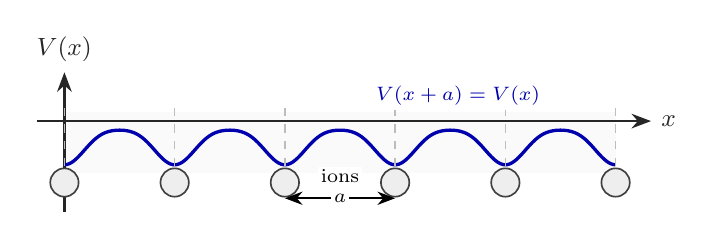
\begin{tikzpicture}[
    >=Stealth,
    axis/.style={->, line width=0.9pt, black!85},
    pot/.style={very thick, blue!68!black},
    guide/.style={dashed, gray!52, line width=0.55pt},
    atom/.style={circle, fill=gray!13, draw=black!75, line width=0.6pt, minimum size=3.6mm, inner sep=0pt},
    label/.style={font=\small},
    smalllabel/.style={font=\scriptsize}
]
    \fill[gray!4] (0,-0.66) rectangle (7.0,0.12);
    \draw[axis] (-0.35,0) -- (7.45,0) node[right, label] {$x$};
    \draw[axis] (0,-1.15) -- (0,0.62) node[above, label] {$V(x)$};

    \draw[pot, domain=0:7.0, samples=240]
        plot (\x,{-0.30 - 0.22*cos(360*\x/1.4) - 0.035*cos(720*\x/1.4)});

    \foreach \x in {0,1.4,2.8,4.2,5.6,7.0} {
        \draw[guide] (\x,-0.78) -- (\x,0.25);
        \node[atom] at (\x,-0.78) {};
    }

    \draw[<->, line width=0.75pt] (2.8,-0.98) -- node[smalllabel, fill=white, inner sep=1pt] {$a$} (4.2,-0.98);
    \node[smalllabel, blue!68!black, fill=white, inner sep=1.5pt] at (5.0,0.32) {$V(x+a)=V(x)$};
    \node[smalllabel, fill=white, inner sep=1pt] at (3.5,-0.70) {ions};
\end{tikzpicture}
\end{document}
